%%%%%%%%%%%%%%%%%%%%%%%%%%%%%%%%%%%%%%%%%
% a0poster Portrait Poster
% LaTeX Template
% with University Copenhagen logo
% Version 1.0 (22/06/13)
%
% Based on:
% The a0poster class was created by:
% Gerlinde Kettl and Matthias Weiser (tex@kettl.de)
%
% This template has been downloaded from:
% http://www.LaTeXTemplates.com
%
%%%%%%%%%%%%%%%%%%%%%%%%%%%%%%%%%%%%%%%%%
% cd /disks/PROJECT/Mickael/COMMUNICATION/SFD2015/;
% pdflatex PosterSFD.tex; bibtex PosterSFD; pdflatex PosterSFD.tex; pdflatex PosterSFD.tex;
% evince PosterSFD.pdf

%----------------------------------------------------------------------------------------
%	PACKAGES AND OTHER DOCUMENT CONFIGURATIONS
%----------------------------------------------------------------------------------------

\documentclass[a0,portrait]{a0poster}
\usepackage[utf8]{inputenc}

\usepackage{multicol} % This is so we can have multiple columns of text side-by-side
\columnsep=100pt % This is the amount of white space between the columns in the poster
\columnseprule=3pt % This is the thickness of the black line between the columns in the poster
\usepackage[margin=3cm]{geometry}
\usepackage[svgnames]{xcolor} % Specify colors by their 'svgnames', for a full list of all colors available see here: http://www.latextemplates.com/svgnames-colors

\usepackage{times} % Use the times font
%\usepackage{palatino} % Uncomment to use the Palatino font

\usepackage{graphicx} % Required for including images
\graphicspath{{figures/}} % Location of the graphics files
\usepackage{booktabs} % Top and bottom rules for table
\usepackage[font=large,labelfont=bf]{caption} % Required for specifying captions to tables and figures
\usepackage{amsfonts, amsmath, amsthm, amssymb} % For math fonts, symbols and environments
\usepackage{wrapfig} % Allows wrapping text around tables and figures
\definecolor{ku}{RGB}{144,26,30}
\definecolor{ku-yellow}{RGB}{255,249,25}

% \usepackage{eso-pic}
               % \newcommand\BackgroundIm{
               % \put(66,-71){
               % \parbox[b][\paperheight]{\paperwidth}{%
               % \vfill
               % \centering
               % \includegraphics[height=\paperheight,width=\paperwidth,keepaspectratio]{background.pdf}%
               % \vfill
               % }}}

\usepackage[english, francais]{babel}
\selectlanguage{francais}

\begin{document}
% \AddToShipoutPicture*{\BackgroundIm}
\Large
%----------------------------------------------------------------------------------------
%	POSTER HEADER
%----------------------------------------------------------------------------------------

% The header is divided into two boxes:
% The first is 75% wide and houses the title, subtitle, names, university/organization and contact information
% The second is 25% wide and houses a logo for your university/organization or a photo of you
% The widths of these boxes can be easily edited to accommodate your content as you see fit



\begin{minipage}[t]{0.60\linewidth}
\vspace{2cm}
\Huge \color{ku} \textbf{Détection de Nouveaux Variants Génomiques \\Simultanément Associés au Glucose Sanguin \\et à la Survenue du Diabète de Type 2} \color{Black}\\ % Title
% \huge\textit{An Exploration of Complexity}
\\ % Subtitle
\Large \textbf{Mickaël CANOUIL}\\[0.5cm] % Author(s)
\Large Génomique Intégrative et Modélisation des Maladies Métaboliques (CNRS UMR 8199)\\ % University/organization
\Large Université de Lille 2\\[0.4cm] % University/organization
\end{minipage}
%
\begin{minipage}[t]{0.40\linewidth}
\vspace{2cm}
\flushright
\color{DarkSlateGray}
\Large \textbf{Information de Contact:}\\
CNRS UMR8199 - Institut de Biologie de Lille\\
1 Rue du Professeur Calmette\\
BP 245\\
F-59019 LILLE CEDEX\\[1cm]
Téléphone : +33(0)3-20-87-11-07\\ % Phone number
Email: \texttt{mickael.canouil@cnrs.fr}% Email address
\end{minipage}

\vspace{1cm} % A bit of extra whitespace between the header and poster content

%----------------------------------------------------------------------------------------

\begin{multicols}{2} % This is how many columns your poster will be broken into, a portrait poster is generally split into 2 columns

%----------------------------------------------------------------------------------------
%	ABSTRACT
%----------------------------------------------------------------------------------------
% \color{ku} % Navy color for the abstract
% \begin{abstract}
% \end{abstract}


%----------------------------------------------------------------------------------------
%	INTRODUCTION
%----------------------------------------------------------------------------------------
% \color{SaddleBrown} % SaddleBrown color for the introduction
\color{DarkSlateGray}
\section*{Introduction}
L'essor des études d'association pangénomiques (GWAS) ont permis l'identification de très nombreux variants génétiques associés à des traits métaboliques et au diabète de type 2 (DT2), notamment 65 loci associés au risque de DT2. En outre, ces loci ont permis de souligner quelques différences physiopathologiques entre l’homéostasie du glucose dans la population générale normoglycémique et les mécanismes moléculaires conduisant au DT2. Néanmoins, ces études se sont restreintes aux données mesurées à un seul temps (données transversales), ainsi aucun variant n'a pu être simultanément associé aux trajectoires temporelles (données longitudinales) du glucose sanguin et au risque de DT2.
% \color{DarkSlateGray} % DarkSlateGray color for the rest of the content


%----------------------------------------------------------------------------------------
%	OBJECTIVES
%----------------------------------------------------------------------------------------
\color{SaddleBrown} % SaddleBrown color for the introduction
\section*{Objectif}
L’objectif principal consiste en la découverte de nouveaux loci simultanément associés à la trajectoire temporelle du glucose sanguin et à l’incidence du diabète de type 2 (Figure \ref{Fig1}).
\color{DarkSlateGray} % DarkSlateGray color for the rest of the content
\begin{center}\vspace{2cm}
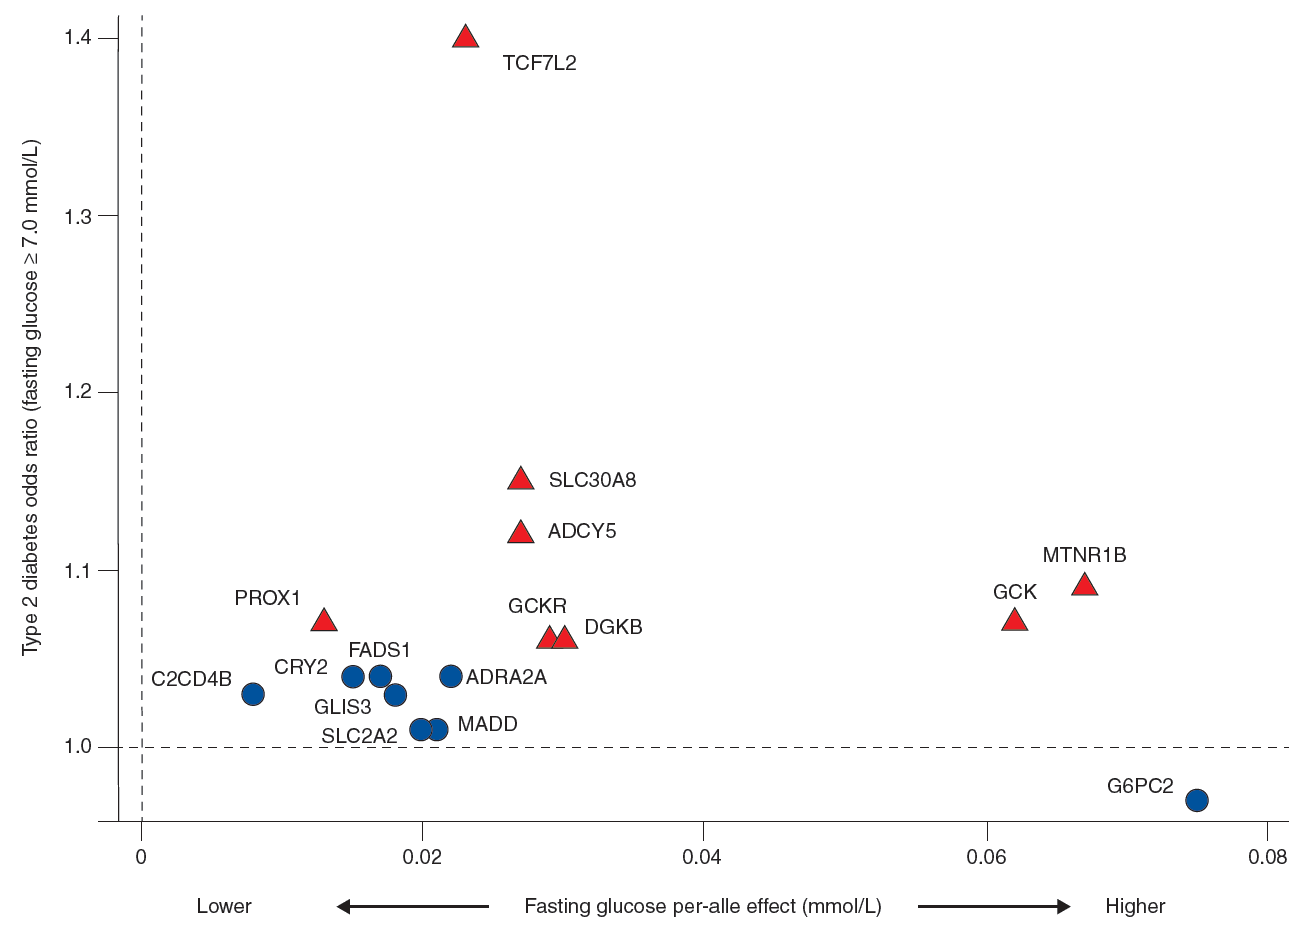
\includegraphics[width=0.8\linewidth]{Yaghootkar.png}
\captionof{figure}{\color{Green} (adaptée de \cite{yaghootkar2013}). Pour chacun des 16 variants génétiques les plus fortement associés à la glycémie à jeun, graphique de la taille de l’effet (en mmol/L) et du rapport de cotes (odds ratio) correspondant pour le diabète de type 2.}
\label{Fig1}
\end{center}%\vspace{1cm}


%----------------------------------------------------------------------------------------
%	MATERIALS AND METHODS
%----------------------------------------------------------------------------------------
\section*{Méthodes}
Nous proposons une approche statistique basée sur un modèle joint \cite{tsiatis2004} qui confrontera la vision actuelle selon laquelle les gènes impliqués dans les niveaux de glucose chez les individus normoglycémiques diffèrent de ceux observés dans les niveaux pathologiques des sujets atteints de DT2.
Le modèle joint pourra être développé à partir d'un modèle linéaire mixte (données longitudinales du glucose) et d'un modèle de survie de Cox (incidence DT2).
\\
\\
Cette approche sera implémentée selon trois composantes, l'effet du SNP sur:
\begin{itemize}
\item la trajectoire temporelle du glucose sanguin ($\gamma $),
\item l'incidence du diabète ($\alpha $),
\item la trajectoire temporelle du glucose sanguin et l'incidence du diabète simultanément ($\beta\gamma+\alpha $),
\end{itemize}
\vspace{1cm}
avec $X(t)$ la trajectoire temporelle du glucose sanguin (Figure~\ref{Fig2}).
% \vspace{2cm}
\begin{center}\vspace{2cm}
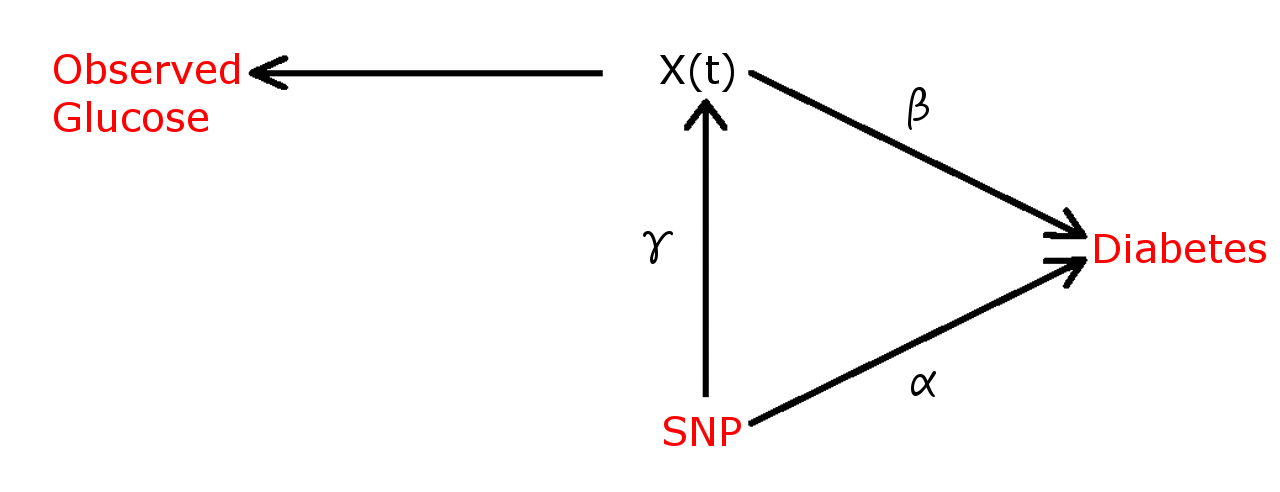
\includegraphics[width=0.8\linewidth]{jointModel.png}
\captionof{figure}{\color{Green} (adaptée de \cite{ibrahim2010}). Diagramme causal pour le modèle joint.
$X(t)$:~trajectoire du glucose sanguin inférée à partir des observations longitudinales;\newline
$\alpha$:~effet du SNP sur le diabète;\newline
$\gamma$:~effet du SNP sur la trajectoire du glucose sanguin;\newline
$\beta$:~effet du glucose sanguin sur le diabète.}
\label{Fig2}
\end{center}%\vspace{1cm}


%----------------------------------------------------------------------------------------
%	RESULTS
%----------------------------------------------------------------------------------------
\color{SaddleBrown} % SaddleBrown color for the conclusions to make them stand out
\section*{Résultats attendus}
Une application de l’approche par modèle joint dans le cadre d’une étude de type GWAS pourrait représenter une percée importante dans la génétique des maladies métaboliques : cette modélisation statistique innovatrice pourrait permettre l’identification de nouveaux loci impliqués à la fois dans le dérèglement de l’homéostasie du glucose et dans la pathophysiologie du DT2.
\color{DarkSlateGray} % Set the color back to DarkSlateGray for the rest of the content


%----------------------------------------------------------------------------------------
%	CONCLUSIONS
%----------------------------------------------------------------------------------------
\color{DarkSlateGray}
\section*{Contexte de recherche}
L'unité de recherche CNRS UMR 8199 "Génomique Intégrative et Modélisation des Maladies Métaboliques" fondée en 1995 et dirigée par le Dr Phippe Froguel,
offre un contexte de choix pour ce projet. En effet, cette unité s'est distinguée par ses contributions majeures en génétique du diabète et de l'obésité et à sa participation au projet LABEX "European Genomic Institute for Diabetes" (EGID), en 2010.
\\
\\
De plus, cette unité comporte une équipe d'analyse statistique et bioinformatique, dont le Dr Ghislain Rocheleau, également porteur de ce projet, détenteur d'un doctorat en statistique et Maître de Conférence des Universités à l'Université de Lille 2 avec chaire d'excellence en biostatistique.
\\
\\
\color{SaddleBrown}
Direction de thèse: Dr. Ghislain ROCHELEAU \& Dr. Philippe FROGUEL
\color{DarkSlateGray} % Set the color back to DarkSlateGray for the rest of the content


%----------------------------------------------------------------------------------------
%	FORTHCOMING RESEARCH
%----------------------------------------------------------------------------------------
% \section*{Forthcoming Research}


%----------------------------------------------------------------------------------------
%	REFERENCES
%----------------------------------------------------------------------------------------
%\nocite{*} % Print all references regardless of whether they were cited in the poster or not
% \large
% \bibliographystyle{apalike} % apalike
% \bibliography{PosterSFD.bib} % Use the example bibliography file sample.bib


%----------------------------------------------------------------------------------------
%	ACKNOWLEDGEMENTS
%----------------------------------------------------------------------------------------
% \section*{Acknowledgements}


%----------------------------------------------------------------------------------------

\end{multicols}
\large
\bibliographystyle{apalike} % apalike
\bibliography{PosterSFD.bib} % Use the example bibliography file sample.bib
\begin{center}
\vfill
{\hspace{2.5cm}
\includegraphics[height=8cm, keepaspectratio]{figures/logo_cnrs.pdf} \hspace{10cm} 
\includegraphics[height=8cm, keepaspectratio]{figures/UL2-WEB-2014.png} \hspace{10cm} 
\includegraphics[height=8cm, keepaspectratio]{figures/logo_egid.pdf}}
\end{center}
\end{document}
